\chapter{Debugging Mode}
The debug mode allows the user to view and/or manipulate the program's internal state for the purpose of debugging. The software allows step wise or block wise line monitor with both forward and backward traversal facility. \Cref{fig:debug:click,fig:debug:hash,fig:debug:run_time,fig:debug:pc} illustrates how users can use this feature in their own instruction set.
\begin{figure}[htbp]
	\centering 
	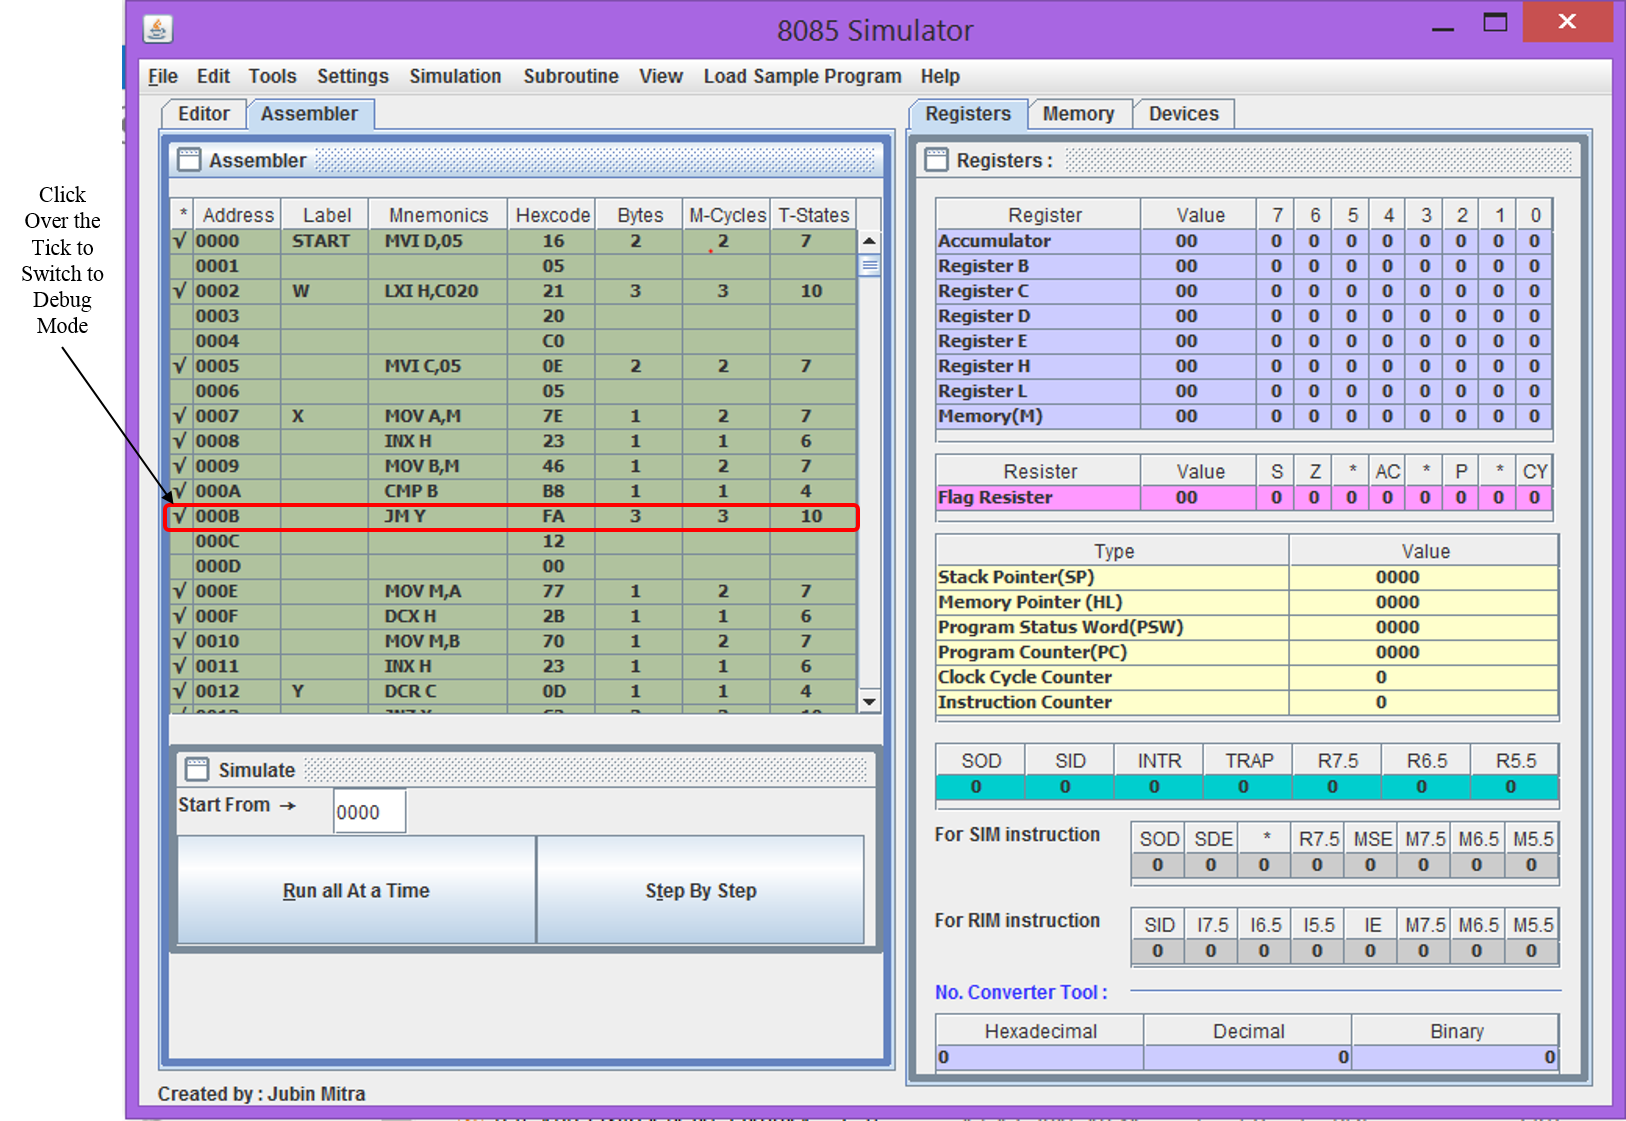
\includegraphics[width=0.9\linewidth]{./Debug_1.png}
	\caption{To Enter into debug mode click on the tick mark}
	\label{fig:debug:click}
\end{figure}

\begin{figure}[htbp]
	\centering 
	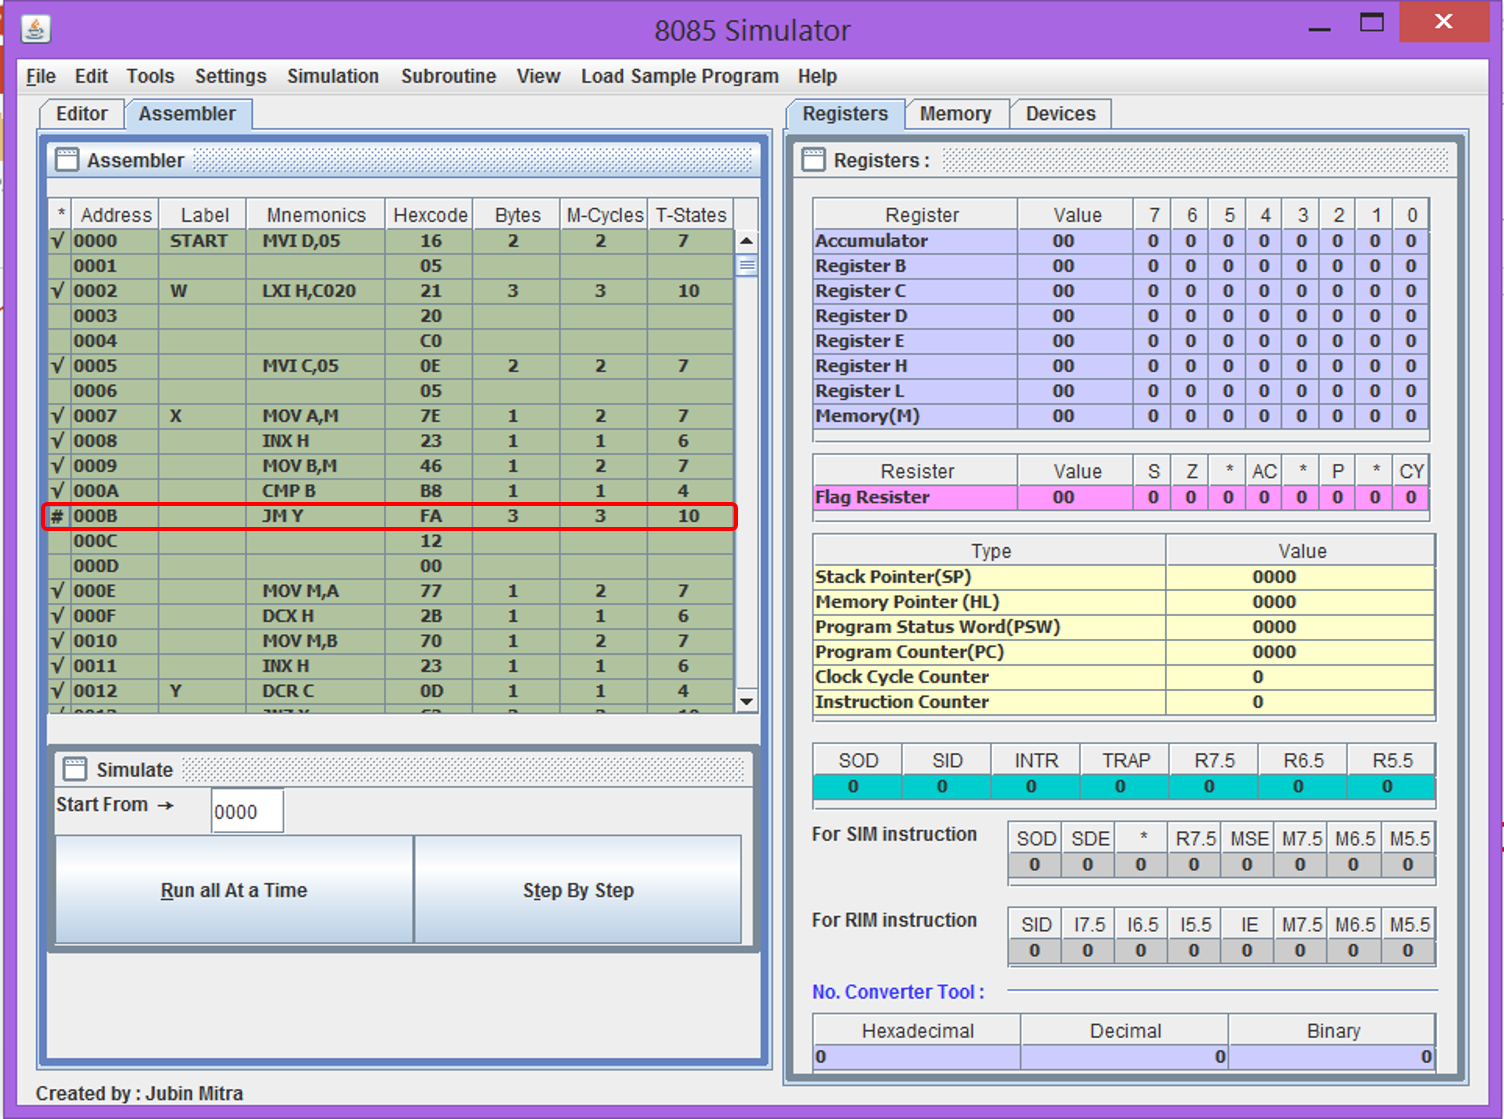
\includegraphics[width=0.9\linewidth]{./Debug_2.png}
	\caption{Figure shows the line is now marked with ` \#' (HASH) character and it is ready to go into debuuging mode during execution of the line}
	\label{fig:debug:hash}
\end{figure}

\begin{figure}[htbp]
	\centering 
	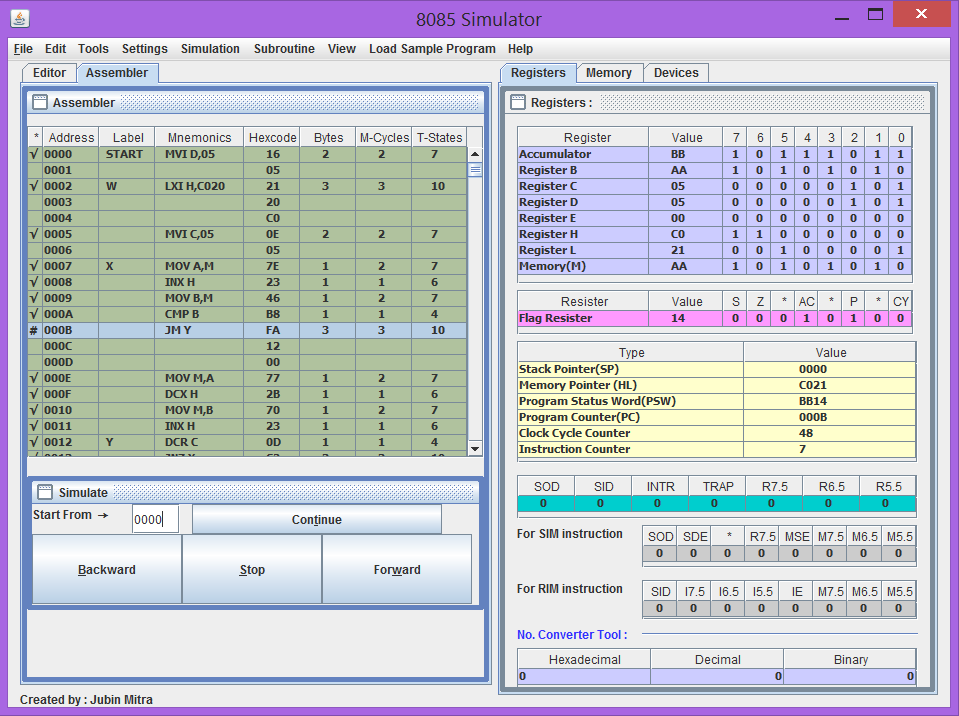
\includegraphics[width=0.9\linewidth]{./Debug_3.png}
	\caption{During run-time the simulation engine stops at marked line and switches to debug mode}
	\label{fig:debug:run_time}
\end{figure}

\begin{figure}[htbp]
	\centering 
	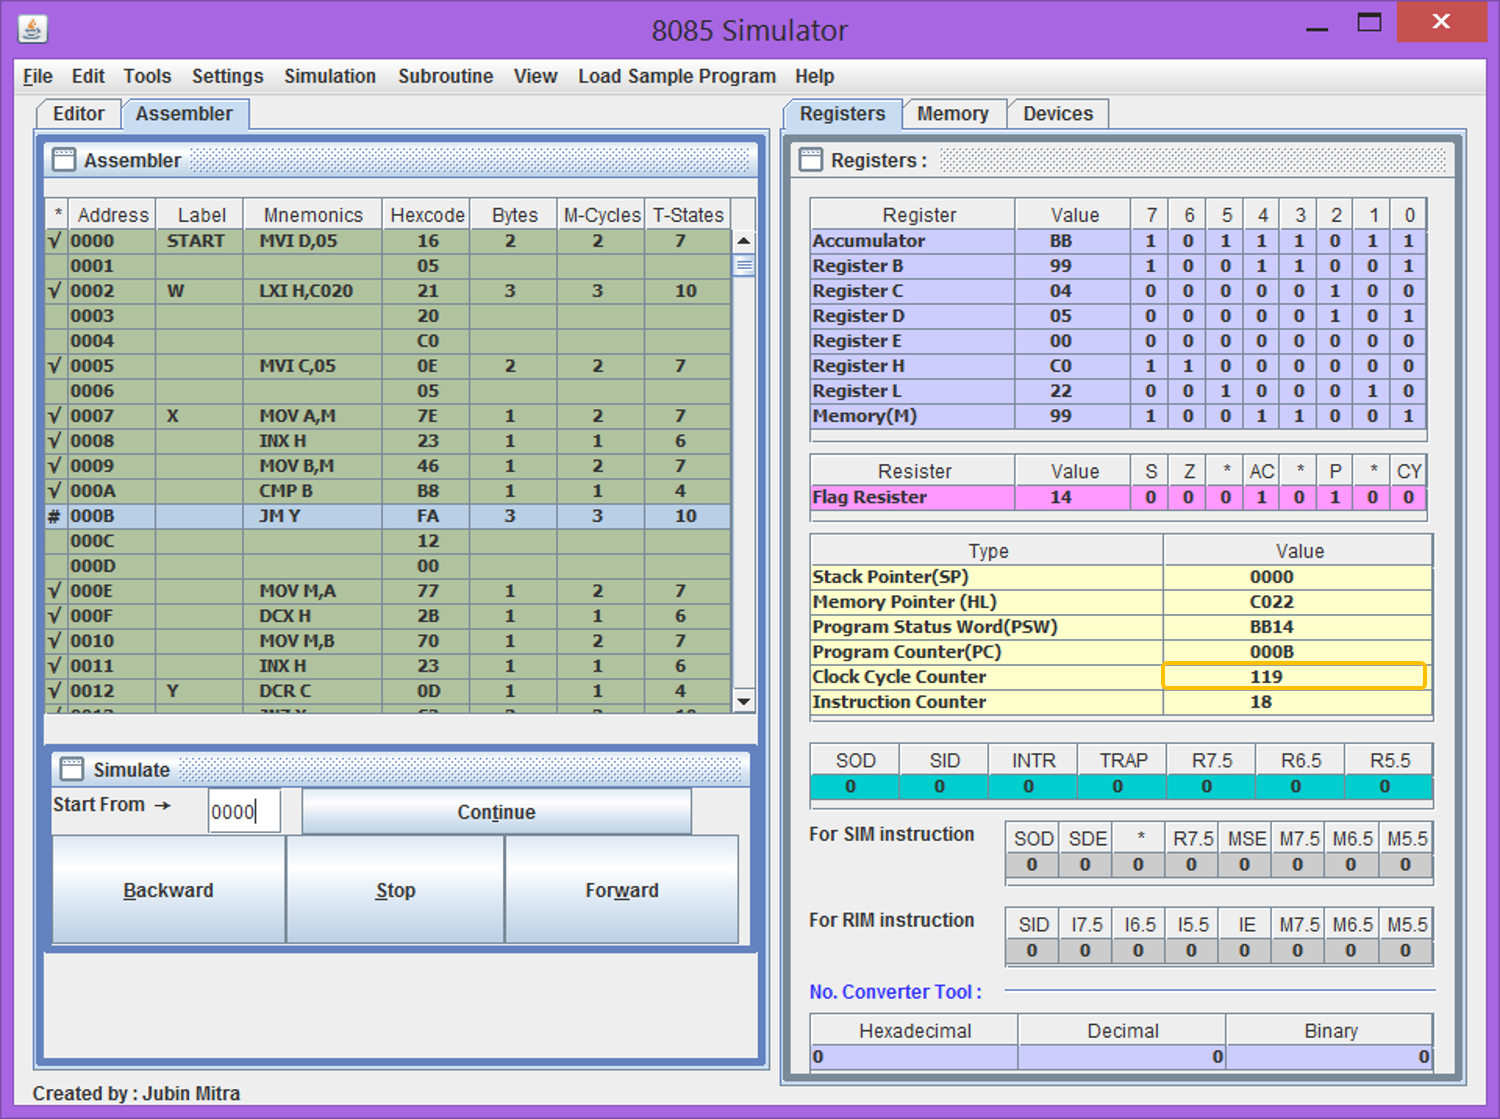
\includegraphics[width=0.9\linewidth]{./Debug_4.png}
	\caption{On pressing ` Continue ' the simulator debugger engine steps over it on next halt. In the figure the changes are marked by ` Program Counter (PC) ' register}
	\label{fig:debug:pc}
\end{figure}

